\section{Les textes}
\subsection{De l'écrit au binaire}
\begin{frame}{Du texte au(x) glyphe(s)}
  \begin{itemize}
  \item Les écrits sous forme d'images ne sont pas exploitables;
  \item L'écriture est donc simplifiée pour ne retenir que les
    \emph{caractères} les uns à la suite des autres ($\neq$
    \emph{lettres});
    \begin{center}
      \begin{tikzpicture}
        \tikzstyle{every node}=[fill=solarizedRebase02,rounded corners]
        \tikzstyle{xlabel}=[fill=solarizedRebase0,fill opacity=30,text opacity=1]
        \tikzstyle{normally}=[very thick]
        \node (a) at (0,0) {Glyphe};
        \node (b) at (4,1.5) {Nombres}
        edge  [<->,normally] node[xlabel,above,sloped] {police} (a);
        \node (c) at (4,0) {Caractère}
        edge  [<->,normally] node[xlabel] {jeu de caractères} (b);
        \node (d) at (4,-1.5) {Touches}
        edge  [<->,normally] node[xlabel] {méthode de saisie} (c);
        \node (d) at (8,0) {Octets}
        edge  [<->,normally] node[xlabel,above,sloped] {encodage} (b);
      \end{tikzpicture}
    \end{center}
  \item Les glyphes sont les dessins des lettres, différents selon les polices
    % \item Différences régionales: ASCII (1968), puis ISO-8859-1 à
    %   ISO-8859-16 (Europe, méditerranée), BIG5 (Chine), Shift-JIS (Japon),
    %   Koi-8R (Russie)...
    % \item Anciennement: encodage trivial sur 8 bits, jeux de caractères
    %   max. 256 caractères;
    % \item Maintenant, Unicode (jeu de caractère) et plusieurs encodages
    %   (UTF8, UTF7, UCS16).
  \end{itemize}
\end{frame}
\begin{frame}{Du caractère au glyphe: la police}
  \begin{itemize}
  \item Les polices supportent souvent plusieurs jeux de caractères. Le
    dessin n'y est stocké qu'une fois.
  \item[\dialogerror] Une même police peut comporter plusieurs glyphes pour le même caractère (formes décoratives)
  \item Une police comporte une partie programme pour sélectionner le dessin le mieux adapté
  \end{itemize}
  \begin{block}{Différence de glyphes}
    La lettre {\Large{$\mathcal{A}$}} et {\Large{A}} représentent le
    même caractère mais pas le même que $\Alpha$.

    De même le \emph{a} de \emph{Abba}, de {\fontfamily{qag}\selectfont
      Abba} ou \textsc{Abba} ou \textrm{Abba} sont les mêmes caractères.
  \end{block}

  \begin{block}{Ligatures esthétiques ou linguistiques}
    La lettre {\Large\OE{}} (ligature linguistique) est différente de
    {\Large{OE}}. La lettre {\textrm{\Large f{}i}} représente deux caractères,
    avec affichage \textrm{\Large{fi}} (ligature esthétique pour éviter le
    \textrm{\Large{f\kern -1pt i}}).

    En arabe ou sanskrit, la ligature est obligatoire (linguistique):
    % \<al-salAm `alaykum> contre \<a l s a l A m ` a l a y k u m>
    \novocalize
    \<tUnis> contre \<t |U n s>.

    La ligature esthétique apparaît au niveau des polices, la ligature
    linguistique au niveau des caractères.
  \end{block}
\end{frame}
\begin{frame}[fragile]{Qu'est-ce qu'un caractère?}
  \begin{itemize}
  \item Au début: lettres, chiffres, ponctuation simplifiée.
  \item[\dialogsystem] Correspondait grossièrement à une touche de
    machine à écrire (+Majuscule/Minuscule)
  \item Au fur et à mesure, de très nombreux caractères ont été rajoutés.
  \item Jeu de caractères universel: Unicode.
  \end{itemize}
  \begin{block}{Quelques caractères dont vous ne connaissez peut-être pas les noms}
    \begin{tabular}{>{\ttfamily}ccll}
      C & Usuel & Français & Anglais\\\hline
      \# & dièse & croisillon, octothorpe & hash, number sign\\
      \& & et & esperluette, et commercial & ampersand, and\\
      | & ou, \emph{païpe} & barre verticale & pipe\\
      / & slash & barre oblique & slash\\
      @ & \emph{arobasse} & arobase & at, at sign\\
      \textbackslash & backslash & contre-oblique & backslash\\
      \_ & underscore & (blanc) souligné & underscore\\
      \verb|[]| & crochets & crochets & (square) brackets\\
      \verb|{}| & accolades & accolades & (curly) braces\\
    \end{tabular}
  \end{block}
\end{frame}
\begin{frame}[label=jeucaractere]{Jeux de caractères}
  \begin{itemize}
  \item Plusieurs jeux de caractères primitifs sur 7 ou 8 bits par caractère.
  \item Un seul a vraiment survécu: ASCII    \begin{presentationonly}\hfill\hyperlink{ascii}{\beamergotobutton{Voir la table}}\end{presentationonly}
    % \item[\dialogwarning] \emph{Byte} anciennement parfois 7 bits. Maintenant systématiquement 8 bits.
  \item Création de jeux de caractères nationaux
  \item Normes ISO-8859-*: caractères 0 à 127 = ASCII; caractères 128 à 255 = caractères locaux
  \item Autres méthodes: KOI-8R (russe), JIS (Japonais), BIG5 (Chinois)... collections de caractères
  \item Universalisation: Unicode: plus de  \numprint{100000} caractères.
  \item[\dialogwarning] Certains caractères sont dupliqués pour des raisons
    historiques
  \end{itemize}
\end{frame}
\begin{exercice}
  \begin{exercicelet}{La table ASCII}
    Trouvez dans la table ASCII:
    \begin{enumerate}
    \item Le caractère de code 0x41
    \item Le caractère de code 0x30
    \item Le caractère \emph{a} et \emph{A}. Comparez l'écriture binaire des codes numériques correspondants.
    \item Le caractère de code 0x20. Quel est-il ?
    \item Le caractère \emph{retour chariot} (son nom est NEWLINE ou NL).
    \end{enumerate}
    Comment passe-t-on d'une lettre à la suivante ? D'une majuscule à une
    minuscule ?
  \end{exercicelet}
\end{exercice}
\subsection{Jeux de caractères et codages}
\begin{frame}{Au début était le \emph{byte}}
  \begin{itemize}
  \item Premiers codages: un caractère = un \emph{byte} = 6 à 8 bits
  \item Rapidement \emph{byte} = octet = 8 bits. ASCII sur 8 bits avait un bit
    inutilisé.
  \item Langues asiatiques: pas suffisant.
  \item Codage à décalage: certaines séquences (non rencontrées
    habituellement) permettent de changer de «~zone~» de caractères.
  \item Certaines séquences déclenchent du codage où 1 caractère est codé par
    2 octets.
  \item Rupture de l'égalité 1 octet = 1 caractère
  \item Autres codages: BIG5 est un codage à 2 octets par caractères pour le
    chinois.
  \end{itemize}
\end{frame}
\begin{frame}[fragile]{Le Mojibake}
  L'enveloppe était envoyée à un étudiant russe par une amie
  française qui a recopié son adresse reçue par e-mail. Le logiciel ne
  savait pas lire les caractères cyrilliques (page de code KOI8-R) et
  les a remplacés par les caractères du code ISO-8859-1.
  \begin{columns}
    \begin{column}{0.35\linewidth}
      \centering
      En KOI8-R:\\{
        \fontencoding{T2A}\selectfont
        Россия Москва, 119415\\
        пр.Вернадского, 37,\\
        к.1817-1,\\
        Плетневой Светлане}
      
      \par
      \bigskip

      En ISO-8859-1:\\
      òÏÓÓÉÑ íÏÓË×Á, 119415\\
      ÐÒ.÷ÅÒÎÁÄÓËÏÇÏ, 37,\\
      Ë.1817-1,\\
      ðÌÅÔÎÅ×ÏÊ ó×ÅÔÌÁÎÅ

      \par
      \bigskip

      Le postier a réussi à faire la transformation inverse! (en rouge)

    \end{column}
    \begin{column}{0.65\linewidth}
      \centering

      \small Une enveloppe en krakozyabry
      ({\fontencoding{T2A}\selectfont кракозябры}) (aussi
      Mojibake). 

      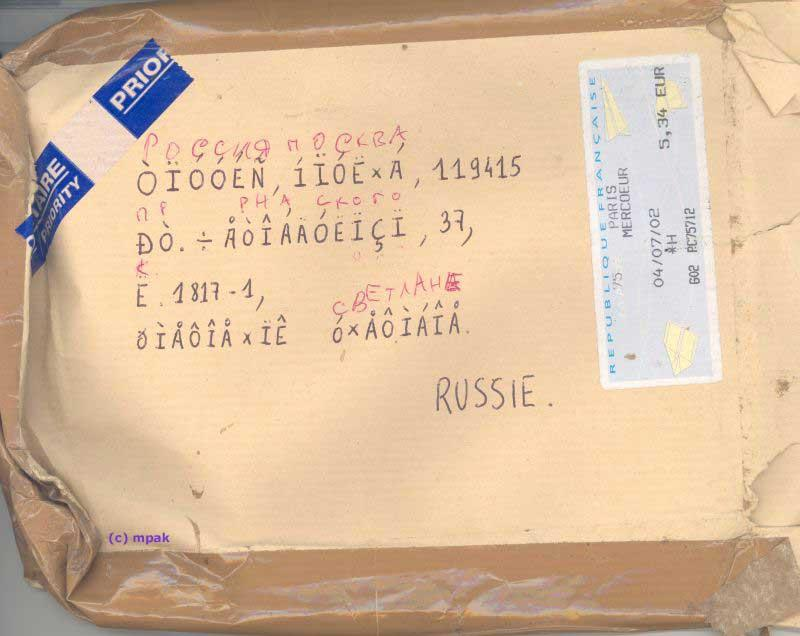
\includegraphics[width=\linewidth]{img/04/mojibake.jpg}
    \end{column}
  \end{columns}
\end{frame}
\begin{exercice}
  \begin{exercicelet}{Codage nationaux et Mojibake}
    Soit le texte : \textrm{Coefficient marée trop fort pour livraison tomates
      cœur-de-bœuf}
    \begin{enumerate}
    \item Identifiez dans ce texte les ligatures linguistiques et les ligatures esthétiques
      \begin{xcorrection} Le \oe est une ligature linguistique (la seule en
        français avec le æ, beaucoup plus rare). Le ffi de coefficient est une
        ligature esthétique. Notez que le oe de coefficient n'est pas une
        ligature.
      \end{xcorrection}
    \item Est-il possible de représenter ce texte dans le jeu de caractères
      ASCII ?
      \begin{xcorrection}
        Non, à cause du \oe. Le \oe n'est d'ailleurs pas une lettre en
        français; par contre le ch en espagnol l'est (voir n'importe quel
        dictionnaire tchèque, où ch n'est pas entre cg et ci, mais juste après
        hz; c'était aussi le cas en espagnol jusqu'à une réforme en 1994).
      \end{xcorrection}
    \item Dans le jeu de caractère ISO-8859-15 (dit \emph{latin-9}), il est
      possible de coder ce texte. Chaque caractère est alors codé par un
      octet unique. Quelle est la taille du fichier qui contient uniquement
      ce texte ?\begin{correction}85 octets (et non 86)\end{correction}
    \item Un polonais lit sur son vieil ordinateur le texte précédent. Il
      voit qu'une des lettres a été remplacée par \H{~} (c'est un double
      accent aigu, comme dans Erd\H{o}s, et pas un tréma comme dans
      Gwenaël). Laquelle et pourquoi ? S'il renvoie le texte tel quel a son
      correspondant français du début, que verra le français et pourquoi ?
      \begin{xcorrection}
        En vérité, il y a de bonnes chances qu'il lise son texte comme étant
        du ISO-8859-2, et non pas du ISO-8859-15, donc il verra un double
        accent aigu à la place de sa lettre. Mais le contenu du fichier est
        inchangé ; s'il est renvoyé au français, le texte apparaîtra normalement.

        L'encodage d'un fichier ne peut pas être deviné simplement comme ça
        (il faut faire une analyse des mots pour déterminer la langue et donc
        l'encodage probable).

        NB: bien sûr, il peut y avoir des problèmes ; les logiciels de
        courrier indiquent parfois l'encodage des pièces jointes, même s'il
        a été mal deviné ; certains éditeurs de texte sauvegardent les
        textes dans un encodage différent de celui qui a été deviné pour
        l'ouverture... bref, les problèmes peuvent exister. Mais le fichier
        n'est a priori pas modifié sauf logiciels qui ne fonctionnent pas
        bien.
      \end{xcorrection}
    \end{enumerate}
  \end{exercicelet}
\end{exercice}
\begin{frame}{Unicode et UTF-8}
  \begin{itemize}
  \item Unicode est une collection de plus de \numprint{100000} caractères qui
    ne spécifie pas la façon de le représenter par une séquence d'octets. La
    taille maximale est de $17\times 2^{16}$ et le code maximal 0x10FFFF
  \item UTF-8 est une façon de transformer un numéro en une séquence d'octets
    \begin{center}\renewcommand{\tabcolsep}{1mm}
      \begin{tabular}{|c|c|c|c|}\hline
        Valeurs & Écriture binaire & Codage UTF-8 (binaire) & octets\\\hline
        0x0--0x7F & abc\,defg & 0abc\,defg & 1 \\
        0x80--0x7FF & abc\,defg\,hijk & 110a\,bcde~10fg\,hijk & 2 \\
        0x800--0xFFFF & abcd\,efgh\,ijkl\,mnop & 1110\,abcd~10ef\,ghij~10kl\,mnop & 3 \\
        0x10000--0x1FFFFF& a\,bcde\,fghi\,jklm\,nopq\,rstu & 1111\,0abc~10de\,fghi~10jk\,lmno~10pq\,rstu &	4 \\\hline
      \end{tabular}
    \end{center}
  \item UCS-2 est un codage partiel sur 2 octets par caractères (représente les $2^{16}$ premiers caractères)
  \item UTF-16 est un codage plus simple qu'UTF-8 utilisant 2 ou 4 octets par
    caractères: 2 pour les premiers, 4 pour les autres (10 octets par paire de
    2 octets).
  \item[\dialoginformation] Avantage de l'UTF-8: économe en place pour l'ASCII (1 octet par caractère)
  \item[\dialogwarning] Inconvénient de l'UTF-8: impossible de dire facilement à quel octet est le n\ieme{} caractère.
  \end{itemize}
\end{frame}
\begin{exercice}
  \begin{exercicelet}{UTF8}
    \def\pres#1{\textcolor{solarizedRed}{\large #1}}
    \def\presg#1{\includegraphics[height=1em]{img/04/#1}}
    \begin{enumerate}
    \item Le caractère de numéro 0x0041 (\pres{A}) est codé par quel(s)
      octet(s) en UTF-8 ?
      \begin{correction}{\texttt{0x41}}\end{correction}
    \item Le caractère de numéro 0x00E9 (\pres{é}) est codé par quel(s)
      octet(s) en UTF-8 ?
      \begin{correction}{\texttt{0xc3 0xa9}}\end{correction}
    \item Le caractère de numéro 0x0F03 (\presg{U0F03}) est codé par quel(s)
      octet(s) en UTF-8 ?
      \begin{correction}{\texttt{0xe0 0xbc 0x83}} C'est le caractère GTER
        YIG MGO 'IM GTER SHEG MA en tibétain (à vos souhaits).\end{correction}
    \item Le caractère de numéro 0x12084 (\presg{U12084}) est codé par quel(s)
      octet(s) en UTF-8 ?
      \begin{correction}{\texttt{0xf0 0x92 0x82 0x84 (4 octets)}} C'est le
        caractère DOUN en cunéiforme (babylonien).\end{correction}
    \item Dans un fichier codé en UTF-8, on trouve les six octets
      suivants. Combien de caractères sont réellements codés dans ce texte ?
      \centerline{\mbox{\large\texttt{0xE6 0x9D 0x8c 0xDE 0xBC 0x43}}}
      \begin{xcorrection}{3 caractères (un sur trois octets, un sur deux, un
          sur un)

          Ce code a l'avantage que l'on peut aussi trouver facilement en lisant
          une suite d'octets représentant de l'UTF-8 combien d'octets occupe
          chaque caractère codé: on les écrit en binaire, et on sait
          automatiquement avec le premier octet dans quelle ligne on se trouve, et
          donc combien d'octets sont utilisés pour le caractère. On peut alors
          sauter au caractère suivant facilement.
        }\end{xcorrection}
    \item {\small L'anglais n'utilise que des caractères dont le numéro est dans la
        première ligne, et est codé traditionnellement en ISO-8859-1 (1
        caractère = 1 octet). Le français utilise 5\% de caractères de la
        deuxième ligne (le reste de la première), et est codé pareil (1
        caractère = 1 octet). L'arabe (le russe, l'hébreu, le grec) sont aussi
        codés traditionnellement par 1 caractère = 1 octet, et comportent 95\%
        de caractères de la deuxième ligne (le reste de la première ligne). Le
        chinois, en revanche est traditionnellement codé en BIG5 (1 caractère
        = 2 octets). Les textes chinois sont à 99\% des caractères de la
        troisième ligne (le reste de la première ligne).}
      
      Pour un texte de 1000 caractères codé en UTF-8, combien d'octets
      seront utilisés en moyenne pour un texte anglais, français, russe et
      chinois ?
      \begin{correction}{ Anglais: 1000 octets. Français: 1050
          octets. Russe: 1950 octets. Chinois: 2980 octets.
        }\end{correction}
    \item Quel est en chinois l'augmentation de la taille du
      texte par rapport au codage traditionnel ?
      \begin{correction}{$(2980-2000)/2000=980/2000=49\%$}\end{correction}
    \end{enumerate}
  \end{exercicelet}
\end{exercice}
\subsection{Les chaînes de caractères}
\def\printit#1#2\relax{\ifx*#1\relax\node (node\x)
  [rectangle,draw,dashed,solarizedRed] at ($(.5,.5)+(\x,0)$) {0x#2}\else\node
  (node\x) at ($(.5,.5)+(\x,0)$) {#1#2} \fi}
\begin{frame}{Les chaînes avec longueur spécifiée}
  Les chaînes de caractères sont des listes ordonnées de caractères.

  Lorsqu'une chaîne de caractères est stockée en mémoire, elle occupe
  plusieurs positions consécutives dans la mémoire. On désigne souvent la
  chaîne par la première position occupée.

  Certains langages résolvent le problème de savoir où la chaîne s'arrête en
  stockant aussi la longueur.

  Problème avec certains codages/jeux de caractères pour trouver le n\ieme{}
  élément d'une chaîne (et en particulier, la longueur en nombre de
  caractères).
  
  Avantage: le calcul de la place mémoire occupée est instantané.

  \begin{example}
    On stocke ici la chaîne «~Allo?~» (le P et la valeur 0x82 sont des
    éléments qui sont dans la mémoire mais ne font pas partie de la chaîne).

    \begin{tikzpicture}
      \draw (-1,0) grid (7,1); \foreach \x/\y in
      {-1/*05,0/A,1/l,2/l,3/o,4/?,5/P,6/*82} { \expandafter\printit\y\relax; }
      \draw
      [decorate,decoration={brace,amplitude=1mm,mirror,raise=1mm},yshift=0pt]
      (0,0)--(5,0); \draw[-latex] (node-1)|-(0,-.5)-|(2.5,-.2);
    \end{tikzpicture}
  \end{example}
  \begin{block}{Est-ce que la longueur est en caractères ou en octets ?}
    En \textbf{octets}, le plus souvent, ou les deux.
    % L'encodage retenu est souvent un encodage où l'un est le multiple de l'autre
    le plus important est de savoir trouver la fin de la chaîne (pour pouvoir
    la copier).
  \end{block}
\end{frame}
\begin{frame}{Les chaînes avec marqueurs de fin}
  Une autre possibilité est de marquer la fin de la chaîne avec un octet
  particulier ou une séquence d'octets particulière.  C'est le cas du langage
  C (et de beaucoup d'autres langages dérivés) qui utilise le caractère nul.
  \begin{example}
    On stocke ici la chaîne «~Allo?~» (le P et la valeur 0x82 sont des
    éléments qui sont dans la mémoire mais ne font pas partie de la chaîne).

    \begin{tikzpicture}
      \draw (0,0) grid (8,1); \foreach \x/\y in
      {0/A,1/l,2/l,3/o,4/?,5/*00,6/P,7/*82} { \expandafter\printit\y\relax; }
      \draw
      [decorate,decoration={brace,amplitude=1mm,mirror,raise=1mm},yshift=0pt]
      (0,0)--(5,0); \draw[-latex] (node5)|-(4,-.5)-|(2.5,-.2);
    \end{tikzpicture}
  \end{example}
  \begin{block}{Est-ce que le marqueur fait partie de la chaîne ?}
    En pratique, oui. Mais il ne fait pas partie du texte codé par la chaîne.

    À l'intérieur d'un langage il n'y a en général qu'une seule sorte de
    chaîne.
  \end{block}
\end{frame}
\begin{frame}{Le problème de l'échappement}
  \begin{block}{La fin de chaîne}
    \begin{itemize}
    \item[\ddialoginformation] Quand la longueur n'est pas spécifiée à côté
      d'une chaîne, la fin de la chaîne est forcément indiquée par une
      séquence spécifique de bits.
    \item S'il existe une séquence spécifique invalide dans le codage pour la
      représentation de caractères, alors on peut la choisir comme
      représentant la fin de chaîne.
    \item Sinon, il faut choisir un caractère qui va coder la fin de la chaîne
    \item[\dialogerror] Comment coder une chaîne qui comporte ce caractère ?
    \end{itemize}
  \end{block}
  \begin{block}{Les séquences signifiantes}
    Parfois, on veut pouvoir utiliser dans des chaînes des séquences qui ont
    un sens spécial. Par exemple, on pourrait vouloir que \texttt{0x0F03}
    représente le caractère 
\includegraphics[height=1em]{img/04/U0F03}\ qu'on
    ne peut pas rentrer facilement au clavier. Mais dans ce cas, comment
    écrire la chaîne \texttt{0x0F03} (comme par exemple pour la phrase «~Si on
    met \texttt{0x0F03} dans une chaîne on obtient le
    caractère 
\includegraphics[height=1em]{img/04/U0F03}~» ?
  \end{block}

  Il faut donc utiliser une procédure d'échappement !
\end{frame}
\begin{frame}{Les séquences d'échappement}
  \begin{itemize}
  \item On utilise une séquence (parfois codante) d'échappement qui permet de
    modifier le sens des caractères qui suivent
  \item Si la séquence d'échappement est codante, on doit prévoir au moins une
    combinaison qui permet de redonner le caractère d'échappement
  \item Avoir des chaînes interprétables complique énormément les opérations
    élémentaires, comme calculer le nombre de caractères dans la chaîne, ou
    savoir si un caractère est présent dans la chaîne.
  \item[\dialogwarning] On se retrouve souvent à «~empiler~» les modes
    d'échappement identiques ou différents.
  \end{itemize}
  \begin{example}
    En langage C et dérivés, le caractère {\textbackslash} est utilisé pour
    introduire des séquences d'échappement.

    \texttt{\textbackslash 0} est le caractère nul.\\
    \texttt{\textbackslash n} est le caractère 10 (NEWLINE).\\
    \texttt{\textbackslash t} est le caractère 9 (TAB).\\
    \texttt{\textbackslash xxx} est le caractère de numéro octal xxx.\\
    \texttt{\textbackslash Uxxxx} est le caractère unicode de numéro
    hexadécimal xxxx. Ce caractère unicode peut représenter plusieurs
    octets. Le codage choisi dépend du compilateur et du type de la chaîne.
  \end{example}
\end{frame}
\begin{exercice}
  \begin{exercicelet}{Les échappements en C}\newcounter{cntx}
    Dessinez quelle est la structure en mémoire des chaînes C suivantes?
    Comment sont elles affichés ?    
    \begin{enumerate}
    \item \verb|"Toto"|
    \item \verb|"Bonjour le monde\n"|
    \item \verb|"Acheter:\n\tponey\n\tporte-avions\n"|
    \item \verb|"\303\251\n"|
    \item \verb|"\U20AC"| (symbole euro)
    \item \verb|"\0"|\setcounter{cntx}{\value{enumi}}
    \end{enumerate}
    \dialogwarning Une bizarrerie historique du C/C++ fait que certaines séquences sont remplacées avant compilation par d'autres caractères:
    \shorthandoff{?}
    \begin{tabular}{l|ccccccccc}
      Trigraphe & ??( & ??) & ??< & ??> & ??= & ??/ & ??' & ??! & ??-\\\hline
      Remplacement &  \string[ &  \string] &  \{ &  \} &  \string# &  \textbackslash &  \string^ &  \string| &  \string~ \\
    \end{tabular}
    \begin{enumerate}\setcounter{enumi}{\value{cntx}}
    \item \verb|"Hello??!"|
    \item \verb|"Bye??/n"|
    \end{enumerate}
  \end{exercicelet}
\end{exercice}
% \begin{exercice}
%   \begin{exercicelet}{Shell et Echo}
%     TODO: trouver des idées
%     TODO: enlever cet exercice ? Trop tôt ? Trop gros?
%     Qu'affiche la commande \verb|/bin/echo -e '\xC3\xA9'| ?
%     Qu'affiche la commande \verb|/bin/echo -e \\xC3\\xA9| ?
%     Qu'affiche la commande \verb|eval "/bin/echo -e \\\\xC3\\\\xA9"| ?
%   \end{exercicelet}
% \end{exercice}
% Local Variables:
% TeX-master: "archi04"
% TeX-PDF-mode: t
% fill-column: 78
% coding: utf-8-unix
% mode-require-final-newline: t
% mode: latex
% mode: flyspell
% ispell-local-dictionary: "francais"
% End:
